\documentclass{llncs}
\usepackage{times}
\usepackage[T1]{fontenc}

% Comentar para not MAC Users
%\usepackage[applemac]{inputenc}

\usepackage{a4}
%\usepackage[margin=3cm,nohead]{geometry}
\usepackage{epstopdf}
\usepackage{indentfirst}
\usepackage{graphicx}
\graphicspath{{Capturas-Ecra/}}
\usepackage{float}
\usepackage{fancyvrb}
\usepackage{amsmath}
\usepackage{array}
%\renewcommand{\baselinestretch}{1.5}


\begin{document}
\mainmatter
\title{TP3 - Serviço de Resolução de Nomes (DNS)}

\titlerunning{TP3 - Serviço de Resolução de Nomes (DNS)}

\author{Diogo Braga \and João Silva}

\authorrunning{Diogo Braga \and João Silva}

\institute{
University of Minho, Department of  Informatics, 4710-057 Braga, Portugal\\
e-mail: \{a82547,a82005\}@alunos.uminho.pt\\
PL2, Grupo 6
}

\date{}
\bibliographystyle{splncs}

\maketitle

\section{Questões e Respostas}

\subsection{\textbf{Qual o conteúdo do ficheiro /etc/resolv.conf e para que serve essa informação?}}
\textbf{R:} Este ficheiro contém o nome do domínio de procura e os servidores que respondem a este nome. O domínio corresponde ao nome do domínio local. O nameserver é responsável pelo endereço de internet pela qual o \textit{resolver} irá interrogar.

\subsection{\textbf{Os servidores www.google.pt. e www.google.com. têm endereços IPv6? Se sim, quais?}}
\textbf{R:} Como mostra a figura \ref{fig:1b}, realizando o comando \textbf{dig www.google.pt.} é possível verificar que o este servidor possui endereços IPv6. De igual forma, realizando o comando \textbf{dig www.google.com.} é possível concluir que este servidor também possui endereços IPv6. Tais são identificados através do Resource Record \textbf{AAAA}.


\begin{figure}[H]
\begin{center}
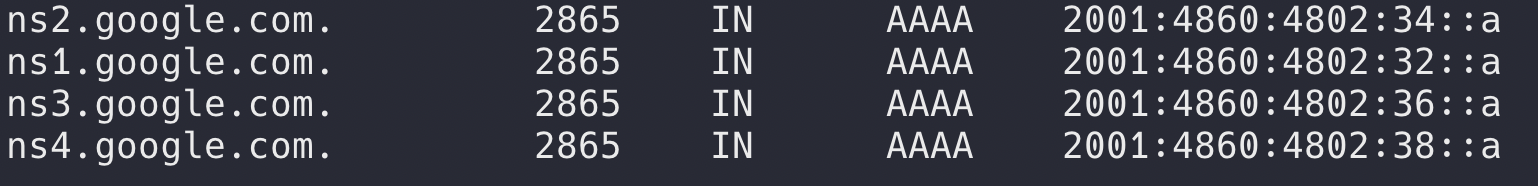
\includegraphics[scale=0.4]{1b.png}
\end{center}
\caption{\label{fig:1b}Resultado da execução do comando \textbf{dig}}
\end{figure}

\subsection{\textbf{Quais os servidores de nomes definidos para os domínios: "ccg.pt.", "pt." e "."?}}
\textbf{R:} Tal como pode ser verificado na figura \ref{fig:1c1}, no domínio \textbf{ccg.pt.}, os nomes definidos para os servidores são \textbf{ns1.ccg.pt.} e \textbf{ns3.ccg.pt.}. Tal é verificável através do Resource Record \textbf{NS}.

\begin{figure}[H]
\begin{center}
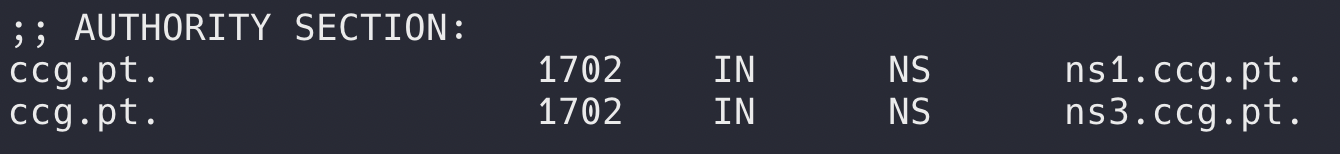
\includegraphics[scale=0.4]{1c1.png}
\end{center}
\caption{\label{fig:1c1}Resultado da execução do comando \textbf{dig}}
\end{figure}

Quanto aos domínios \textbf{pt.} e \textbf{.}, estes não possuem servidores de nomes definidos porque definem o início de uma zona e todos os seus parâmetros. Tal pode ser verificado na figura \ref{fig:1c2} e \ref{fig:1c3}, respetivamente.

\begin{figure}[H]
\begin{center}
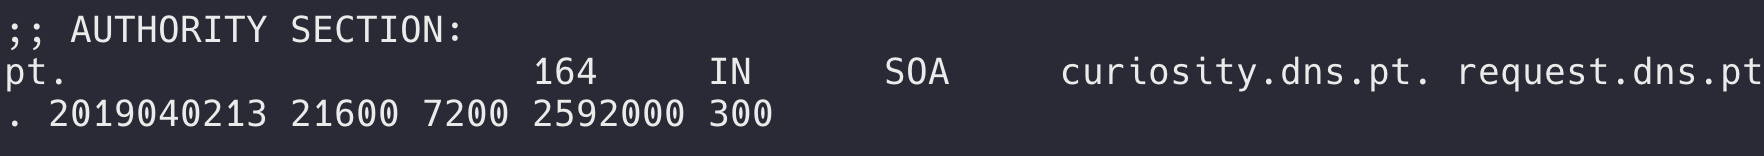
\includegraphics[scale=0.4]{1c2.png}
\end{center}
\caption{\label{fig:1c2}Resultado da execução do comando \textbf{dig}}
\end{figure}

\begin{figure}[H]
\begin{center}
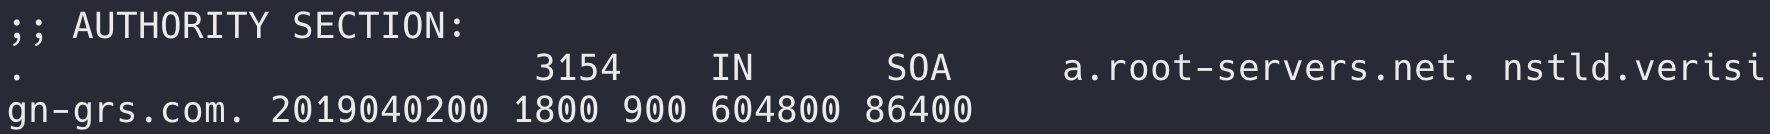
\includegraphics[scale=0.4]{1c3.png}
\end{center}
\caption{\label{fig:1c3}Resultado da execução do comando \textbf{dig}}
\end{figure}


\subsection{\textbf{Existe o domínio eureka.software.? Será que eureka.software. é um host?}}
\textbf{R:}


\subsection{\textbf{Qual é o servidor DNS primário definido para o domínio ami.pt.? Este servidor primário (master) aceita queries recursivas? Porquê?}}
\textbf{R:}


\subsection{\textbf{Obtenha uma resposta "autoritativa" para a questão anterior.}}
\textbf{R:}


\subsection{\textbf{Onde são entregues as mensagens dirigidas a marcelo@presidencia.pt ? E a guterres@onu.org?}}
\textbf{R:}


\subsection{\textbf{Que informação é possível obter acerca de www.whitehouse.gov? Qual é o endereço IPv4 associado?}}
\textbf{R:}


\subsection{\textbf{Consegue interrogar o DNS sobre o endereço IPv6 2001:690:a00:1036:1113::247 usando algum dos clientes DNS? Que informação consegue obter? Supondo que teve problemas com esse endereço, consegue obter um contacto do responsável por esse IPv6?}}
\textbf{R:}


\subsection{\textbf{Os secundários usam um mecanismo designado por "Transferência de zona" para se atualizarem automaticamente a partir do primário, usando os parâmetros definidos no Record do tipo SOA do domínio. Descreve sucintamente esse mecanismo com base num exemplo concreto (ex: di.uminho.pt ou o domínio cc.pt que vai ser criado na topologia virtual).}}
\textbf{R:}


\end{document}
